\section{Chemical and biological processes}\label{se:chemical_process}
This section will analyse the chemical processes that wastewater undergoes from the water is used to it is cleaned at the water treatment plant. The processes in a wastewater treatment plant will be investigated to get an understanding of the different processes. %Furthermore a illustration will be presented to elaborate the details in a sewer. 

Within wastewater there is an infinity number of living organisms before entering the WWTP. It contains from around 100000 to 1000000 microorganisms per millimeter. Theses organisms originates from sanitary waste and soil. They are a natural living part of the organic matter and they are most important in the biological degradation of the waste in the WWTP. The primary reason for a high water quality at the output of the WWTP is to have great understanding of these microorganisms, especially bacteria. A acceptable purification of the wastewater is therefore depended on understanding the requirements for the most optimal conditions for the microorganisms. 

Nearly all of the microorganisms found in wastewater are not harmful and therefore does not cause a disease for men. However a small group of the microorganisms are causing a disease and these are to a great concern for the WWTP. The most known diseases are typhoid fever, dysentery, cholera, and hepatitis.

The microorganisms in WWTP have a specific role in the decomposition of the waste. The three most notable microorganisms in the biological treatment process are bacteria, fungi and protozoa. Where the bacteria have the primary role of degrading the wastewater compounds, thereby producing settable soils. Bacteria is a single cell organism and is capable of reproducing rapidly when in contact with water. They consume the food by taking it through the cell wall. Fungi, like bacteria decompose the organic waste. However they also pose a significant problem for the operation as the fungi can proliferate to an extent that can detrimental consequences for the effluent quality. Lastly protozoa acts as predators to control the bacterial population. 

% https://www.aquaenviro.co.uk/fungal-problems-in-wastewater-treatment-works/ kilde for fungus

In figure \ref{fig:sewer_overview_of_the_chemical_process} an illustration is shown of the processes that wastewater undergoes within the sewer.
\begin{figure}[H]
\centering
\includegraphics[width=1\textwidth]{report/introduction/pictures/detailed_sewer.pdf}
\caption{General overview of a sewer where the potential processes are illustrated. arbejdsblad billede. \fxnote{Ny tegning}}
\label{fig:sewer_overview_of_the_chemical_process}
\end{figure}

Wastewater are subject to a variety of mass changes in a sewer. One is due to free electrons in the wastewater, where different kinds of chemical reactions occurs. This results in different compounds being created which will be elaborated on in subsection \ref{subse:chemical_reactions_in_a_sewer}. The concentration and the chemical compounds that occurs at the inlets of the sewer are changed at the wastewater treatment plant. Furthermore these chemical reactions has the possibility to create gases that is released into the urban atmosphere, which is not ideal as it typically is malodorous. Besides chemical reaction in the sewer there are also microorganisms. %The microorganisms consumes the sludge that sediments in the sewer and by consuming it they help break down the waste into inorganic and organic byproducts \cite{bacteria_sewer}. 
These microorganisms are reproducing on the biofilm that is created on the surface of the pipe. Furthermore the wastewater in the pipes can sink into the groundwater and the soils due to small leaks in the construction of the sewer. The wastewater ends up at the wastewater treatment plant, this process will be explained in subsection \ref{subse:Wastewater treatment plant}. And as previous mentioned in case of heavy precipitation to avoid flooding, the wastewater will be lead into receiving waters. 


\subsection{Chemical reactions in a sewer}\label{subse:chemical_reactions_in_a_sewer}
A wastewater treatment plant does not only receive what is discharged into the sewer from the industry and households but also the chemical and microbial reactions that occurs in a sewer. The chemical reactions occur as redox reactions between the different compounds. Redox reaction is the transfer of electrons between two compounds at a atomic or molecular scale. By transferring electrons from one compound to another new compounds will arise, such as hydrogen sulfide which is know for its malodorous smell of rotten eggs. These reactions are determined by the electron acceptors that are present in the wastewater. The electron acceptor is the compound that receives electrons in a redox reaction. Examples of dissolved acceptors are oxygen ($O_2$), nitrate ($NO^-_3$) and sulfate ($SO^{2-}_4$), which determines whether aerobic, anoxic or anaerobic processes may occur. The redox reaction reduces these three compounds in the wastewater by changing them to new compounds such as water $H_2O$, molecular nitrogen ($N_2$) and hydrogen sulfide ($H_2S$) \cite{Sewer_processes}. 

Redox reactions are determined to a great extend by the design of the sewer where different conditions such as aerobic, anaerobic and anoxic conditions exist. The last only occurs if nitrate is artificially added to the wastewater. If nitrate is added to the wastewater, then the bacteria can survive in sewers where there are no oxygen. If the process is aerobic the typical characteristics for the sewer are either partly filled gravity sewer or an aerated pressure sewer. This means that there are free oxygen ($O^+$) molecules, and these will be connected with hydrogen to create water. If the process is anoxic, which occurs in pressure sewers, then the addition of nitrate to the wastewater results in molecular nitrogen. In an anaerobic sewer the characteristic of the sewer is either a pressure sewer or a full flowing gravity sewer, then the redox reaction will result in hydrogen sulfide. Thereby sewers can actively be designed to achieve a specific process \cite{Sewer_processes}. 


This knowledge is used to construct a simulation that is able to express the chemical and microbial reaction which occur in wastewater. %A general model for describing the processes within a sewer is a extremely complex procedure, due to the variability in modeling, catchment characteristics and climate conditions which in practice are legion and therefore a general model formulation is not optimal. 
To model these chemical and microbial reactions in sewers a model concept, Wastewater Aerobic/Anaerobic Transformation in Sewers (WATS), is used. The WATS model is expressed as differential mass balances equations that is suitable for numerical computations and can therefore be include in simulations for a specific objective e.g. model of water, biofilm and gas phase transformations. The WATS model can be applied to variety of different sewers as long as a fundamental understanding of the sewer process is available, whether it is aerobic, anoxic or anaerobic processes that dominate the sewer, the soil composition and the pH concentration of the wastewater must also be included in the WATS model for a sewer \cite{Sewer_processes}.     



%Furthermore turbulence in the flow of the wastewater affects reaeration and can release odorous and corrosive particles into the atmosphere \cite{Sewer_processes}.    

% \begin{figure}[H]
% \centering
% 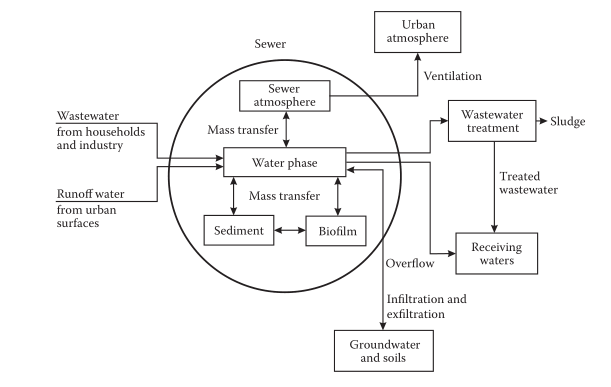
\includegraphics[width=1\textwidth]{report/introduction/pictures/sewer_overview_of_the_different_parts.png}
% \caption{Illustrates how the wastewater flows from the industry and households to the treatment plant. \fxnote{Ny tegning}}
% \label{fig:sewer_overview_of_the_different_parts}
% \end{figure}

\subsection{Wastewater treatment plant}\label{subse:Wastewater treatment plant}
\fxnote{Noget specifikt for hvordan det ser ud i Fredericia}
At the WWTP the wastewater undergoes several process before the chemicals, dirt, etc. is removed from it and is lead back into the nature. The first stage in clearing the wastewater is screening, where larger objects are removed from the wastewater which would block the flow or damage the equipment. Some of the objects that are filtered from the wastewater are bottles, plastic bags and diapers.  %which basically is all items that would either block or damage the equipment. 

Stage two is the primary treatment where the separation of organic matter, among other things human excrements, from the wastewater. By leading the wastewater into a large settlement tank the organic matter will sink to the bottom of the tank. The matter that have sedimented is now called sludge. At the bottom large scrappers are scrapping the floor moving the sludge to the center of the tank where it is pumped away for further treatment. From here the separated water is pumped into the secondary treatment. 

In this stage the water is pumped into large rectangular tanks where air is pumped into the water to make the bacteria consume the sludge that have passed on from the previous stage. When the bacteria have consumed the sludge it will start to sediment at the bottom of the tank. This process takes 3-6 hours.  

After these treatment processes there are still some diseases in the water. If the water is lead in to sensitive or fragile ecosystems the water is further treated. It is disinfected for at least 20-25 minutes in tanks where a mixture of chemicals are used to cleanse the remaining water before leading it into the environment. If the water is not lead to a fragile ecosystem the last phase is passed through a settlement tank where the remaining particles will sediment at the bottom of the tank creating more sludge. From here the water is lead through a filter that remove any additional particles. Hereafter the water is lead into the environment. 

The sludge that is collected in the process undergoes further treatment, where the remaining water in the sludge is separated from it. The water is lead back to the wastewater treatment process where it will undergo the same process again. The sludge is collected and used for agricultural use.





